\documentclass{article}


\usepackage{amsmath,amssymb}
%\usepackage{dsfont} %install texlive-fonts-extra 
\usepackage{tikz}
\usetikzlibrary{bayesnet}

\author{Otto Fabius}
\title{Background layout}
\begin{document}
	
	\maketitle


\section{Variational Inference}
\begin{itemize}
	\item Variational Optimization key idea
	\item Often used for inference problems, decompose the log marginal according to Bishop (eq 10.2)
	\item 
\end{itemize}
Variational Inference methods in general are used when data $\mathbf{X}$ is assumed to be generated through some process from an underlying set of stochastic latent variables $\mathbf{Z}$. The probability of data is therefore modeled as $p(\mathbf{X}) = p(\mathbf{Z}|\mathbf{X})p(\mathbf{Z})$. Moreover, this set of methods is used when the true posterior $p(Z|X)$ can not be evaluated analytically. Variational Bayes introduces a tractable distribution $q(\mathbf{\mathbf{Z}|\mathbf{X}})$ as an approximation to $p(\mathbf{Z}|\mathbf{X}))$.
\\
More on Variational Inference....
\section{Bag-of-words Topic Modelling}

\subsection{LSI and pLSI}
\subsection{LDA}\label{LDA}
Explain LDA following (p)LSI and Variational Inference.
\subsection{Deep Exponential Families}\label{DEF}

Deep exponential families is relevant for this work for two reasons: It shows that deeper models can be more powerful than LDA, and is currently the state of the art. Nothing in our methods depends on this section.


\section{SGVB}\label{sgvb_section}

Discuss requirements of problem scenario for SGVB to be applicable. \\

Notes:\\
- No simplifying assumptions are made about the marginal or posterior probabilities, as is the case in other VB methods (check!!) \\
- $q(\mathbf{Z}|\mathbf{X})$ is not necessarily factorial and its parameters $\phi$ are not computed from some closed-form expectation (as in mean field VI)
- General purpose introduction of sgvb . \\

- areas of success of sgvb.

- compare VAE to LDA:

\subsection{Relation to LDA}

Discuss how closely related Graphical models are. Note that sampling separately for each word could facilitate the extra plate LDA has in a VAE approach, but then not only inefficient but also not possible to learn non-linear dependencies between words.

\begin{figure}\label{LDAVAE GM}
	\centering
	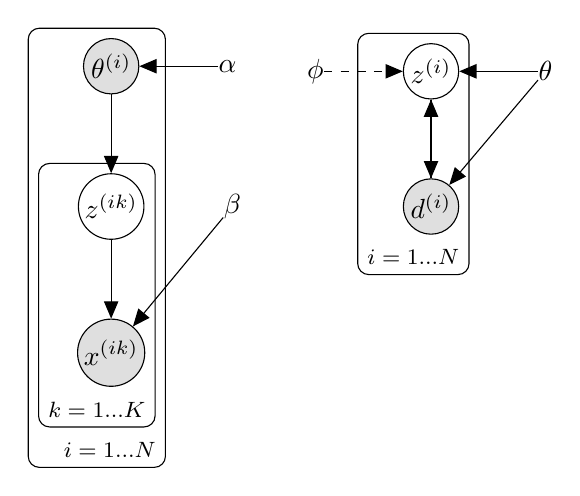
\begin{tikzpicture}[node distance = 1.5cm]
	\node[obs] (x) {$x^{(ik)}$}; 
	
	\node[latent, above=of x] (z) {$z^{(ik)}$}; 
	
	\node[obs, above=of z] (d) {$\theta^{(i)}$}; 
	
	\node[const, right=of d] (a) {$\alpha$} ;
	\node[const, right=of z] (th) {$\beta$} ;
	
	\edge {a} {d};
	\edge {z} {x};
	\edge {d} {z};
	\edge {th} {x};
	
	
	\plate {xz} {(x)(z)} {$k = 1...K$};
	\plate {xzd} {(x)(z)(d)(xz)} {$i = 1...N$};
	
	
	
	\node[const, right=of th] (extra) {};
	\node[obs, right=of extra] (d2) {$d^{(i)}$};
	
	\node[latent, above=of d2] (z2) {$z^{(i)}$};
	
	\node[const, right=of z2] (th2) {$\theta$} ;
	\node[const, left=of z2] (ph2) {$\phi$};
	
	
	\edge {z2} {d2};
	\edge {th2} {z2};
	\edge {th2} {d2};
	\edge [dashed,bend left] {d2} {z2}
	\edge [dashed] {ph2} {z2}
	
	
	
	\plate {zd2} {(z2)(d2)} {$i = 1...N$};
	
	
	\end{tikzpicture}
	\caption{Graphical Model of LDA (left) and VAE Topic Model (left)}
\end{figure}

\subsection{Neural Variational Inference for Topic Models}\label{NVItopic}
NVI Topic Models
\section{Stick-Breaking VAE}\label{sbvae_section}
As detailed in \ref{sgvb_section}, one restriction of SGVB in general is the need for a differentiable, non-centered parametrization of the latent variables. Therefore, e.g. Beta distributed latent variables (as used in e.g. LDA \cite{bleil2003latent}), can not be used in the SGVB framework. \\ Nalisnyck \& Smith extend SGVB to Stick-breaking priors by using the Kumaraswami Distribution as the approximate posterior. The rest of this section \ref{sbvae_section} is not much more than a description of the relevant part of Nalisnyck \& Smyth \cite{nalisnick2016deep}.\\ 
Where other popular topic models such as LDA \cite{blei2003latent} and, to lesser extent, Deep Exponential Families \cite{ranganath2015deep} have binary latent variables with a the VAE approach described in section \ref{TopicVAE} has continuous latent variables. These are assumed to be independent and normally distributed. Using Beta distributed latent variables in a SGVB approach is not possible because, as explained in \ref{sbvae_section}, but we can use a stick-breaking VAE for topic modeling in a similar manner to the topic VAE described in \ref{TopicVAE}. We will therefore describe the model details in the same fashion as we did in \ref{TopicVAE}. \\

\subsection{The Stick-Breaking Process}\label{sb_process}

\subsection{The Kumaraswami Distribution}\label{kum}

	
	
\end{document}



	